\documentclass{beamer}
\usetheme{AnnArbor}
\usecolortheme{dolphin}
\setbeamercolor*{frametitle}{bg=white,fg=structure.fg}
\title{GPU-Accelerated Document Filtering}
\author{Gordon Reid - 1002536r}
\date{25th March 2014}
\begin{document}
\frame{\titlepage}
\frame{\tableofcontents}
\section{Document Classification}
\subsection{Introduction}
\frame{
    \frametitle{Document Classification}
    \begin{itemize}
        \item A problem of growing importance, data centres handle terabytes of
        data daily.
        \item Need fast, but efficient, method of filtering.
        \item Data parallel problem, each document independent from one another.
    \end{itemize}
}
\frame{
    \frametitle{Classification Method}
    \begin{itemize}
        \item Na{\"{\i}}ve Bayes Classifier for plain text documents.
        \item Two classes, A or B. Think spam or not spam.
        \item Profile of interesting terms used to score document terms.
        \item N-Grams of terms also scored. `Rolex' versus `Cheap Real Rolex'.
        \item Documents with a high enough score are given class A, otherwise B.
    \end{itemize}
}
\subsection{Prior Work}
\frame{
    \frametitle{Prior Work}
    \begin{itemize}
        \item Parser for plain text documents documents using a C++ application.
        \item Parser runs on a CPU.
        \item Scoring can be off-loaded to FPGA.
        \item Parsing is bottleneck, 427MB/s. FPGA scores at 749MB/s.
        \item Work looking into parsing and scoring on FPGA.
    \end{itemize}
    This project looks into use of OpenCL and GPUs.
}
\section{OpenCL}
\subsection{Overview}
\frame{
    \frametitle{OpenCL Overview}
    \begin{itemize}
        \item Open Computing Language.
        \item Framework for applications designed for heterogenous platforms.
        \item Can run on CPUs, GPUs, FPGAs, and more.
        \item Roughly a subset of C99.
        \item Host code in C++ which runs on CPU.
        \item Device code, the kernel, in OpenCL which runs on target device.
    \end{itemize}
}
\subsection{OpenCL meets Document Classification}
\frame{
    \frametitle{OpenCL meets Document Classification}
    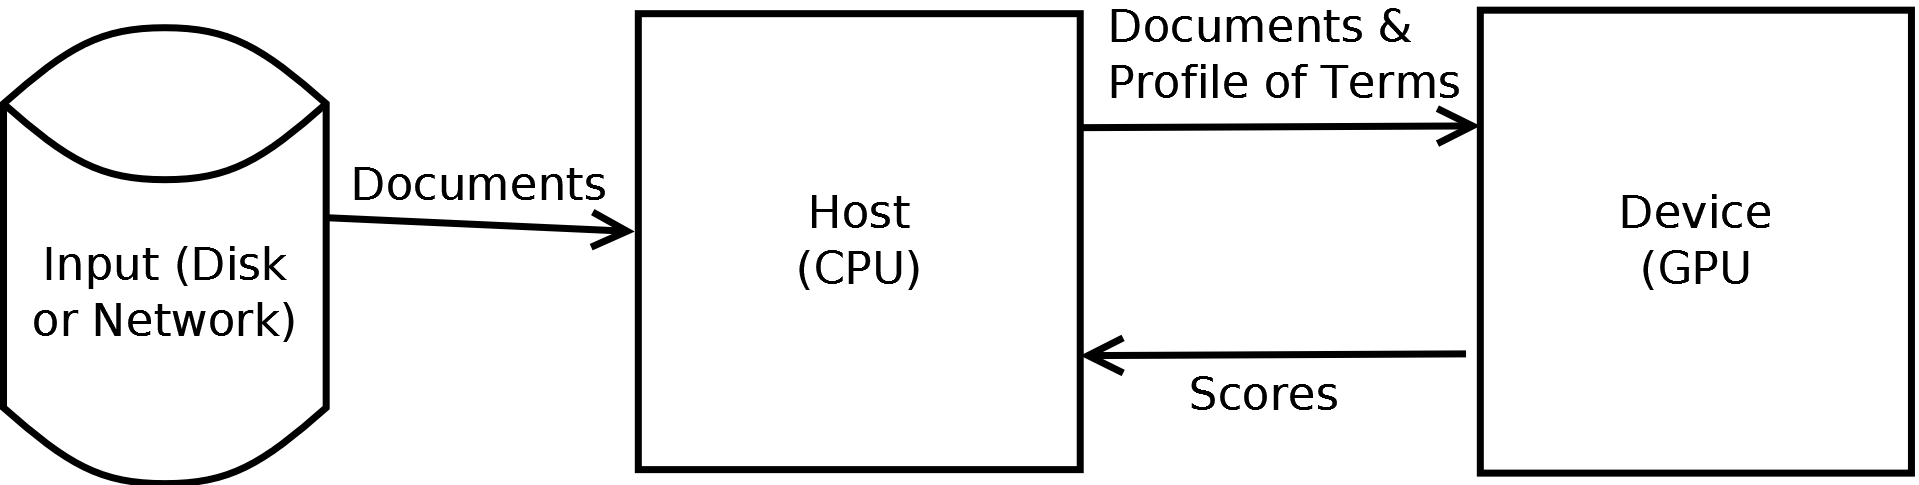
\includegraphics[width=\linewidth]{images/hostDevice.png}
    \begin{itemize}
        \item Host code reads in documents and sets up OpenCL environment.
        \item Device given documents and profile of terms.
        \item Both scoring only, and parsing and scoring kernels.
        \item Host reads back scores from target device.
        \item Document classification output based on score.
        \item Target devices include Tesla C2075 and Intel Xeon Phi 5110P.
    \end{itemize}
}
\section{TREC Data Collection}
\frame{
    \frametitle{TREC Data Collection}
    \begin{itemize}
        \item Text Retrieval Conference document set.
        \item Around 78000 plain text documents.
        \item News articles fitting into seven different categories.
        \item Three selected for one class, four for the other class.
        \item Twelve profiles for each class combination created.
    \end{itemize}
}
\section{Scoring}
\frame{
    \frametitle{Scoring}
    \begin{itemize}
        \item Use a pre-parsed collection of document terms for TREC collection.
        \item OpenCL kernel scores this collection based on profile.
        \item Scores returned back to host.
    \end{itemize}
}
\subsection{Results}
\frame{
    \frametitle{Scoring Results}
    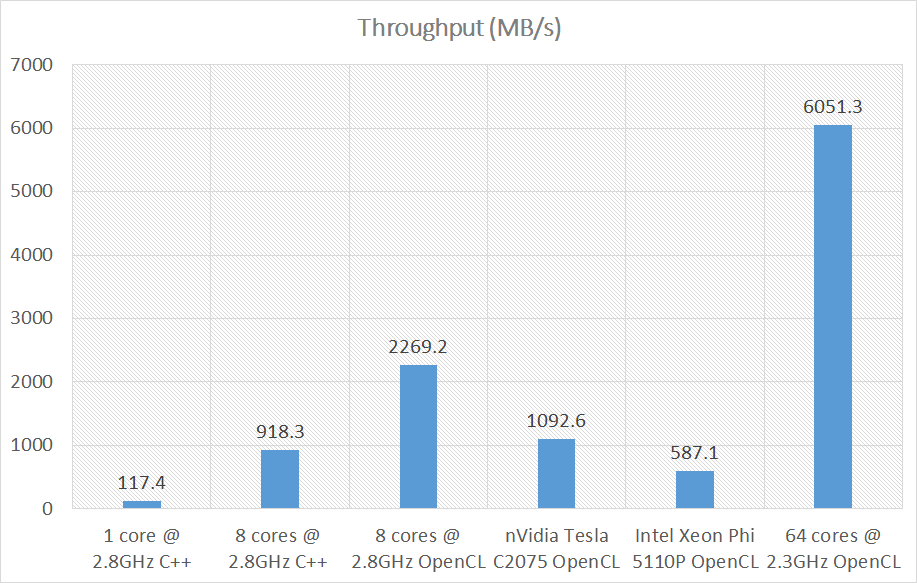
\includegraphics[width=\linewidth,height=\textheight,keepaspectratio]{images/scoringOnlyBest.png}
}
\subsection{Discussion}
\frame{
    \frametitle{Discussion of Results}
    \begin{itemize}
        \item AMD CPU system comes out top. 64 cores at 1.8GHz up to 2.3GHz
        \item Tesla C2075 exceeds 1GB/s. CPU parser would be bottleneck still.
        \item OpenCL on CPU improves performance compared to C++ version.
        \item CPU results for reference only. The CPU would need to also be
        parsing documents so actual scoring throughput would be lower.
        \item Confirms parser and scorer on one device required.
    \end{itemize}
}
\section{Parsing and Scoring}
\frame{
    \frametitle{Parsing and Scoring}
    \begin{itemize}
        \item Use plain text documents, TREC collection.
        \item OpenCL kernel parses documents as well as scoring them based on
        given profile.
        \item Scores returned back to host.
    \end{itemize}
}
\subsection{Results}
\frame{
    \frametitle{Parsing and Scoring Results}
    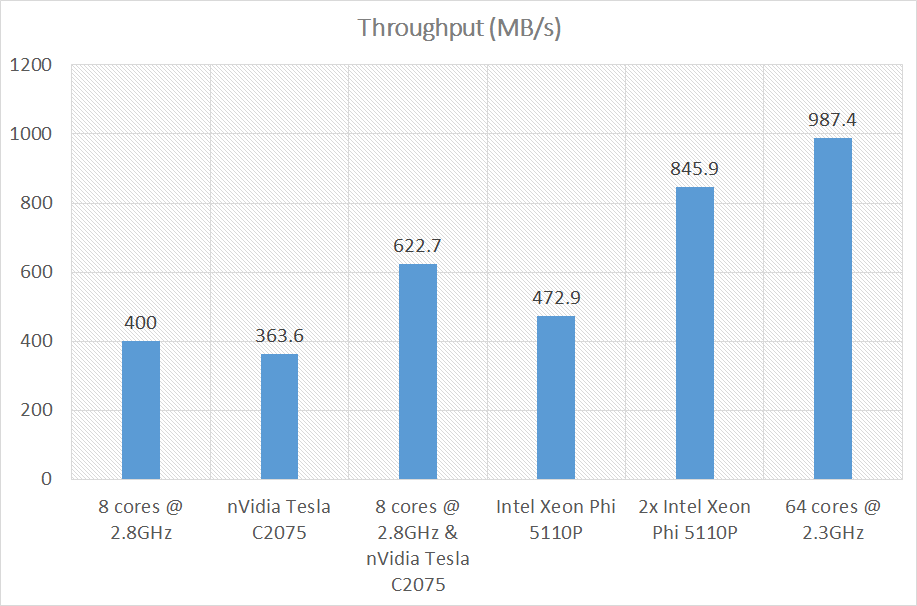
\includegraphics[width=\linewidth,height=\textheight,keepaspectratio]{images/parsingScoringBest.png}
}
\subsection{Discussion}
\frame{
    \frametitle{Discussion of Results}
    \begin{itemize}
        \item AMD CPU system comes out top again at nearly 1GB/s.
        \item Two Intel Xeon Phis a close second. Almost linear scaling compared
        to single Phi.
        \item Dual CPU and GPU system also has near-linear scaling.
        \item All dual device results improve on previous bottleneck of 427MB/s.
        \item 1GB/s result is 8Gbit/s and so could parse 10Gbit/s Ethernet.
        \item With an average throughput of Ethernet of around 30\%, this system
        could parse 30Gbit/s.
    \end{itemize}
}
\section{Conclusion}
\frame{
    \frametitle{Conclusion}
    \begin{itemize}
        \item Document filtering suitable application of OpenCL.
        \item Real time hard drive and solid state disk filtering possible.
        \item GPU acceleration is effective.
        \item Modern, consumer class devices are more efficient.
        \item Adding multiple devices scales well.
    \end{itemize}
}
\end{document}
